\chapter{Reinterpretation}
\label{chap:reinterpretation}

In Section ~\ref{sec:results}, we presented our observed yields in the signal region and found they were consistent with the background expectations. Armed with this information, we were able to set upper limits on the cross sections of the T5HH and T5ZH SMS models (as a function of the gluino mass). As these two models are certainly not the only possibility for new physics to arise, it is important that we provide additional information necessary to cast other models within the context of our analysis. This information allows a model builder to make predictions of the yields for their models of similar construction. They can compare these yields to the ones we observed in our analysis and see if their model has potential for further investigation or would already be ruled out.

We present the efficiencies for mass-tagging and $b\bar{b}$-tagging of Higgs and Z bosons reconstructed as AK8 jets. Tagging efficiencies for the five largest decay modes relevant to the analysis for the H boson are seen in \ref{fig:effH}. Tagging efficiencies for the hadronic decay modes of the Z boson are seen in Figure~\ref{fig:effZ}, the much lower mass tagging efficiency for the Z boson is due to our choice of signal mass window [85, 135 GeV] not being optimal for Z reconstruction. 

In the analysis, each event is categorized depending on the mass and $b\bar{b}$-tagging of the two AK8 jets. Among these combinations, three are related to $b\bar{b}$-tagging: they can both be tagged, one-and-only-one can be tagged, or neither of them can be tagged. There are two relevant combinations for the mass-tagging among the jets: they are both within the signal mass window [85, 135 GeV], or not. On an event-by-event basis, given the $p_{T}$ of the Higgs or Z bosons from the model, we can use the provided efficiency maps to form event weights for each of the 6 analysis bins for the event. As these weights are dependent on the decay mode of the boson, we additionally need to make sure to choose the correct map. The total expected yields in each bin are then obtained by summing these weights over the events in the sample.

\textbf{For each event}, we form ``primitive weights'' which combine the status of the mass and $b\bar{b}$-tagging, these are seen in Table~\ref{tab:evtwht}. j$_{0, bb}$ represents the probability the leading AK8 jet is $b\bar{b}$-tagged, j$_{0, m\text{-}sig}$ represents the probability the leading AK8 jet falls within the signal mass window [85, 135 GeV], and j$_{0, m\text{-}side}$ represents the probability the leading AK8 jet falls within the sideband mass window [50, 85]+[135, 250 GeV].

\begin{table}[hbp!]
\caption{Effective event weights for $b\bar{b}$ and mass tagging of AK8 jets.}
\label{tab:evtwht}
\begin{tabular}{rrl}
\hline\hline
both jets are $b\bar{b}$-tagged & W$_{2b}$ & = $j_{0, b{b}} \cdot j_{1, b{b}}$\\
only one jet is $b\bar{b}$-tagged & W$_{1b}$ & = $j_{0, b{b}} \cdot ( 1 - j_{1, b{b}} ) ~+~ ( 1 - j_{0, b{b}} ) \cdot j_{1, b{b}}$\\
neither jet is $b\bar{b}$-tagged & W$_{0b}$ & = $( 1 - j_{0, bb} ) \cdot ( 1 - j_{1, b{b}} )$\\
both jets are mass-tagged & W$_{m}$ & = $j_{0, m\text{-}sig} \cdot j_{1,m\text{-}sig}$\\
! both jets are mass-tagged & W$_{!m}$ & = $(j_{0, m\text{-}side} \cdot j_{1, m\text{-}sig}) + (j_{1, m\text{-}sig} \cdot j_{1, m\text{-}side}) + (j_{0, m\text{-}side} \cdot j_{1, m\text{-}side})$\\
\hline\hline
\end{tabular}
\end{table}

Now that these weights are formed we can combine them appropriately to make event weights for the individual analysis bins. The weights for a given bin are then summed over the total number of events in the sample. The weights for each analysis bin are shown in Figure \ref{fig:wdiag}.

\begin{figure}[hbp!]
\centering
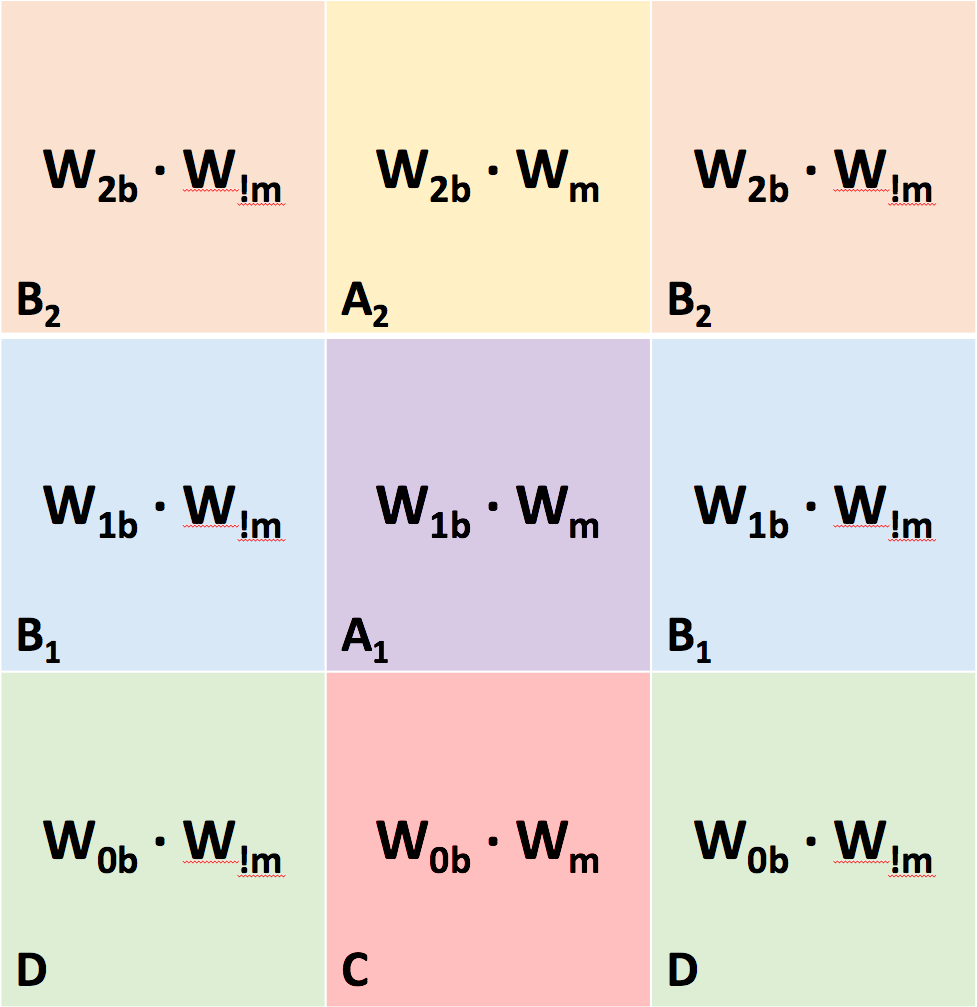
\includegraphics[width=0.4\linewidth]{figs/weights.png}
\caption[Diagram for compiling the weights into each of the 6 analysis bins.]{Diagram for compiling the weights into each of the 6 analysis bins. (See Figure~\ref{fig:abcd})}
\label{fig:wdiag}
\end{figure}

\begin{figure}[hbp!]
\centering
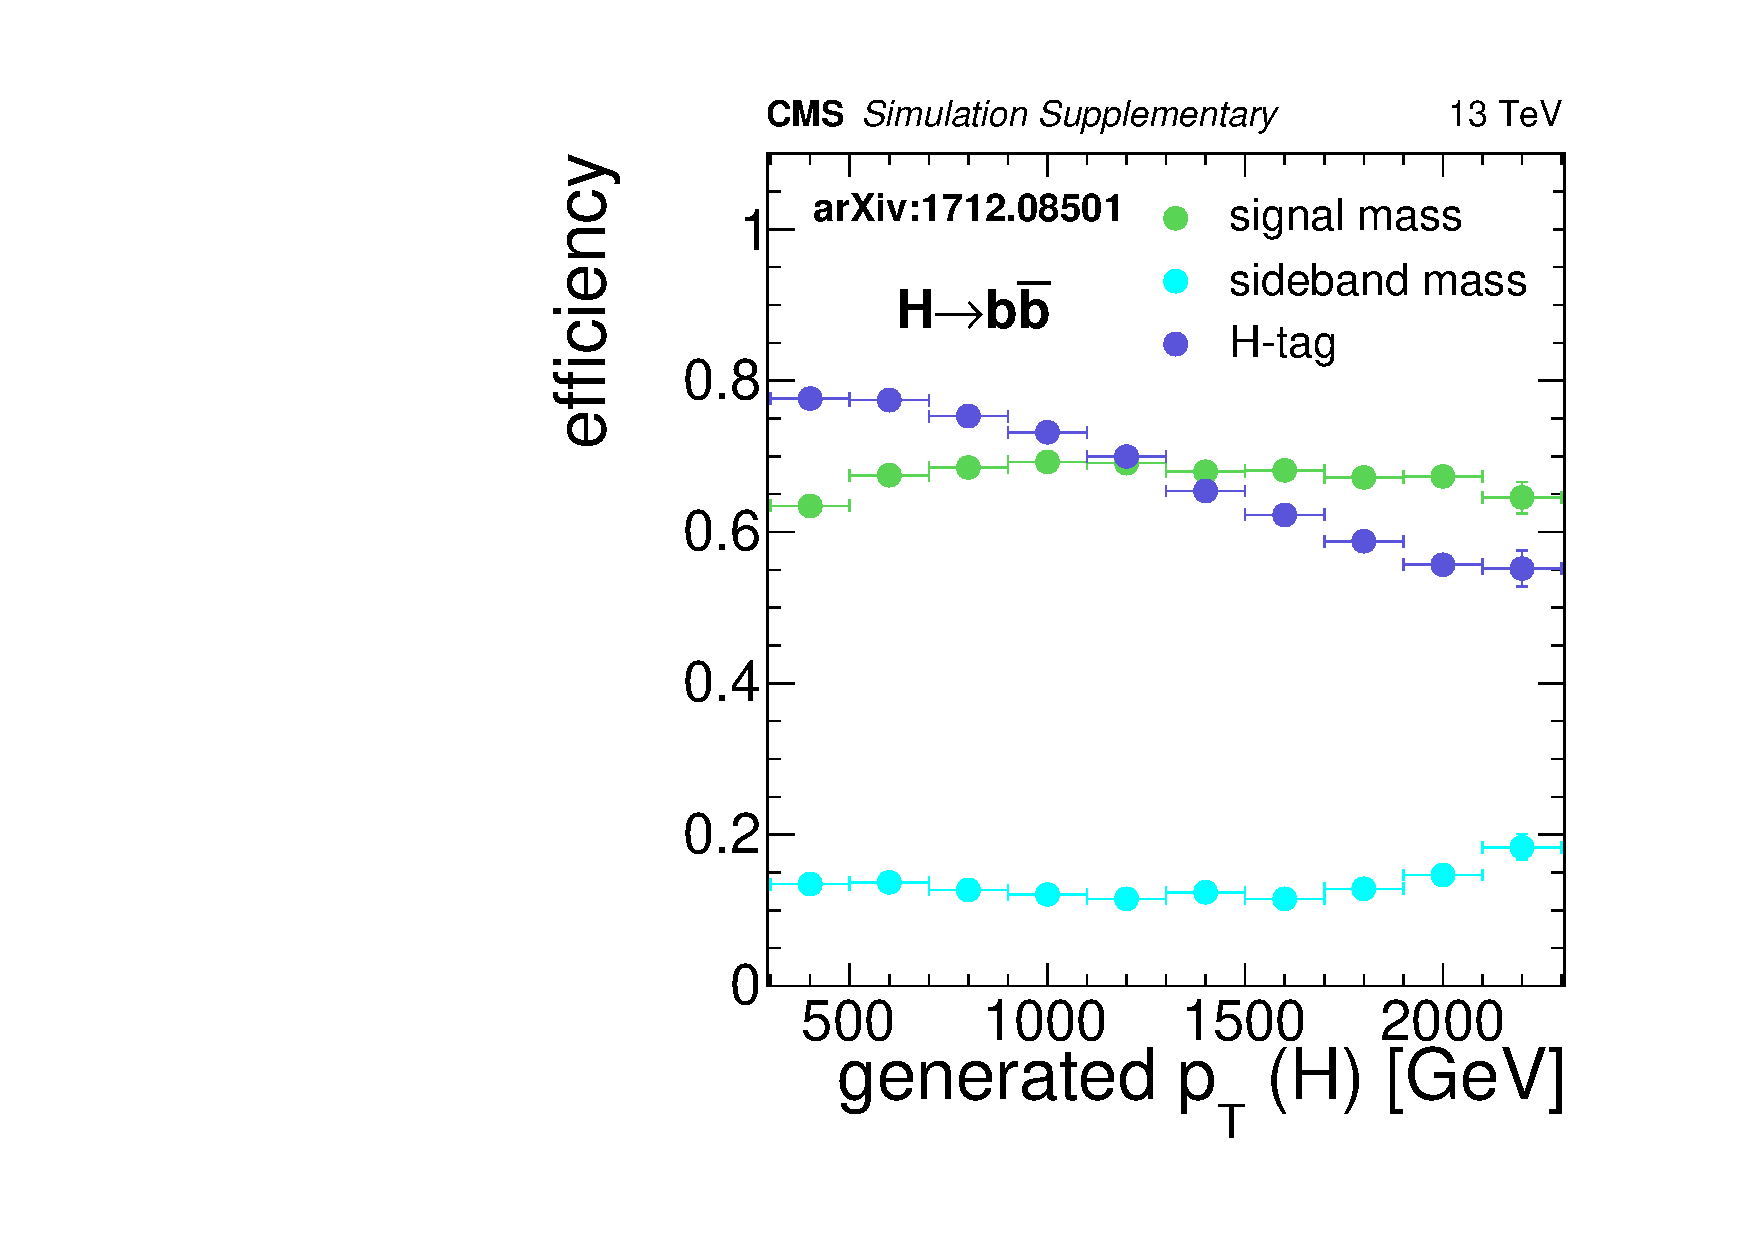
\includegraphics[width=0.425\linewidth]{figs/CMS-SUS-17-006_Figure-aux_006.pdf}
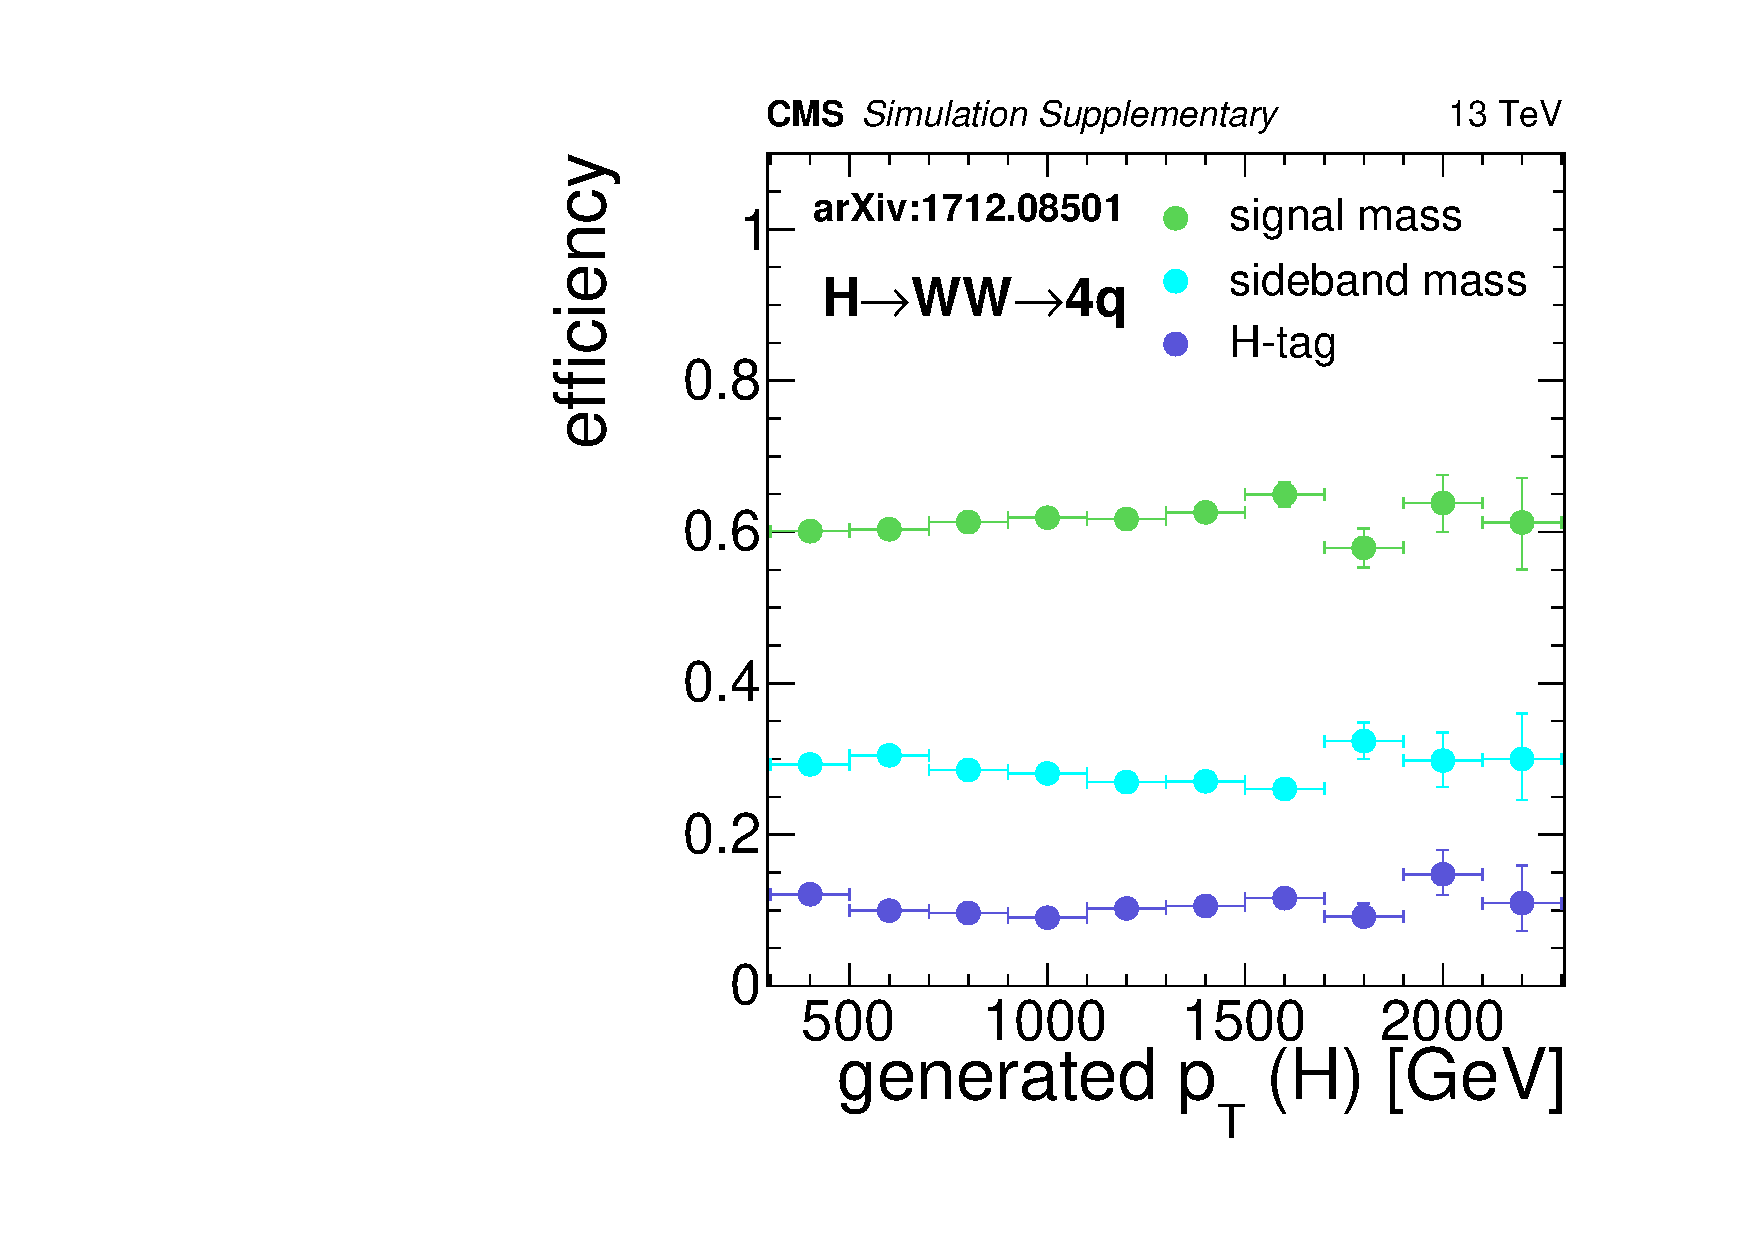
\includegraphics[width=0.425\linewidth]{figs/CMS-SUS-17-006_Figure-aux_007.pdf}
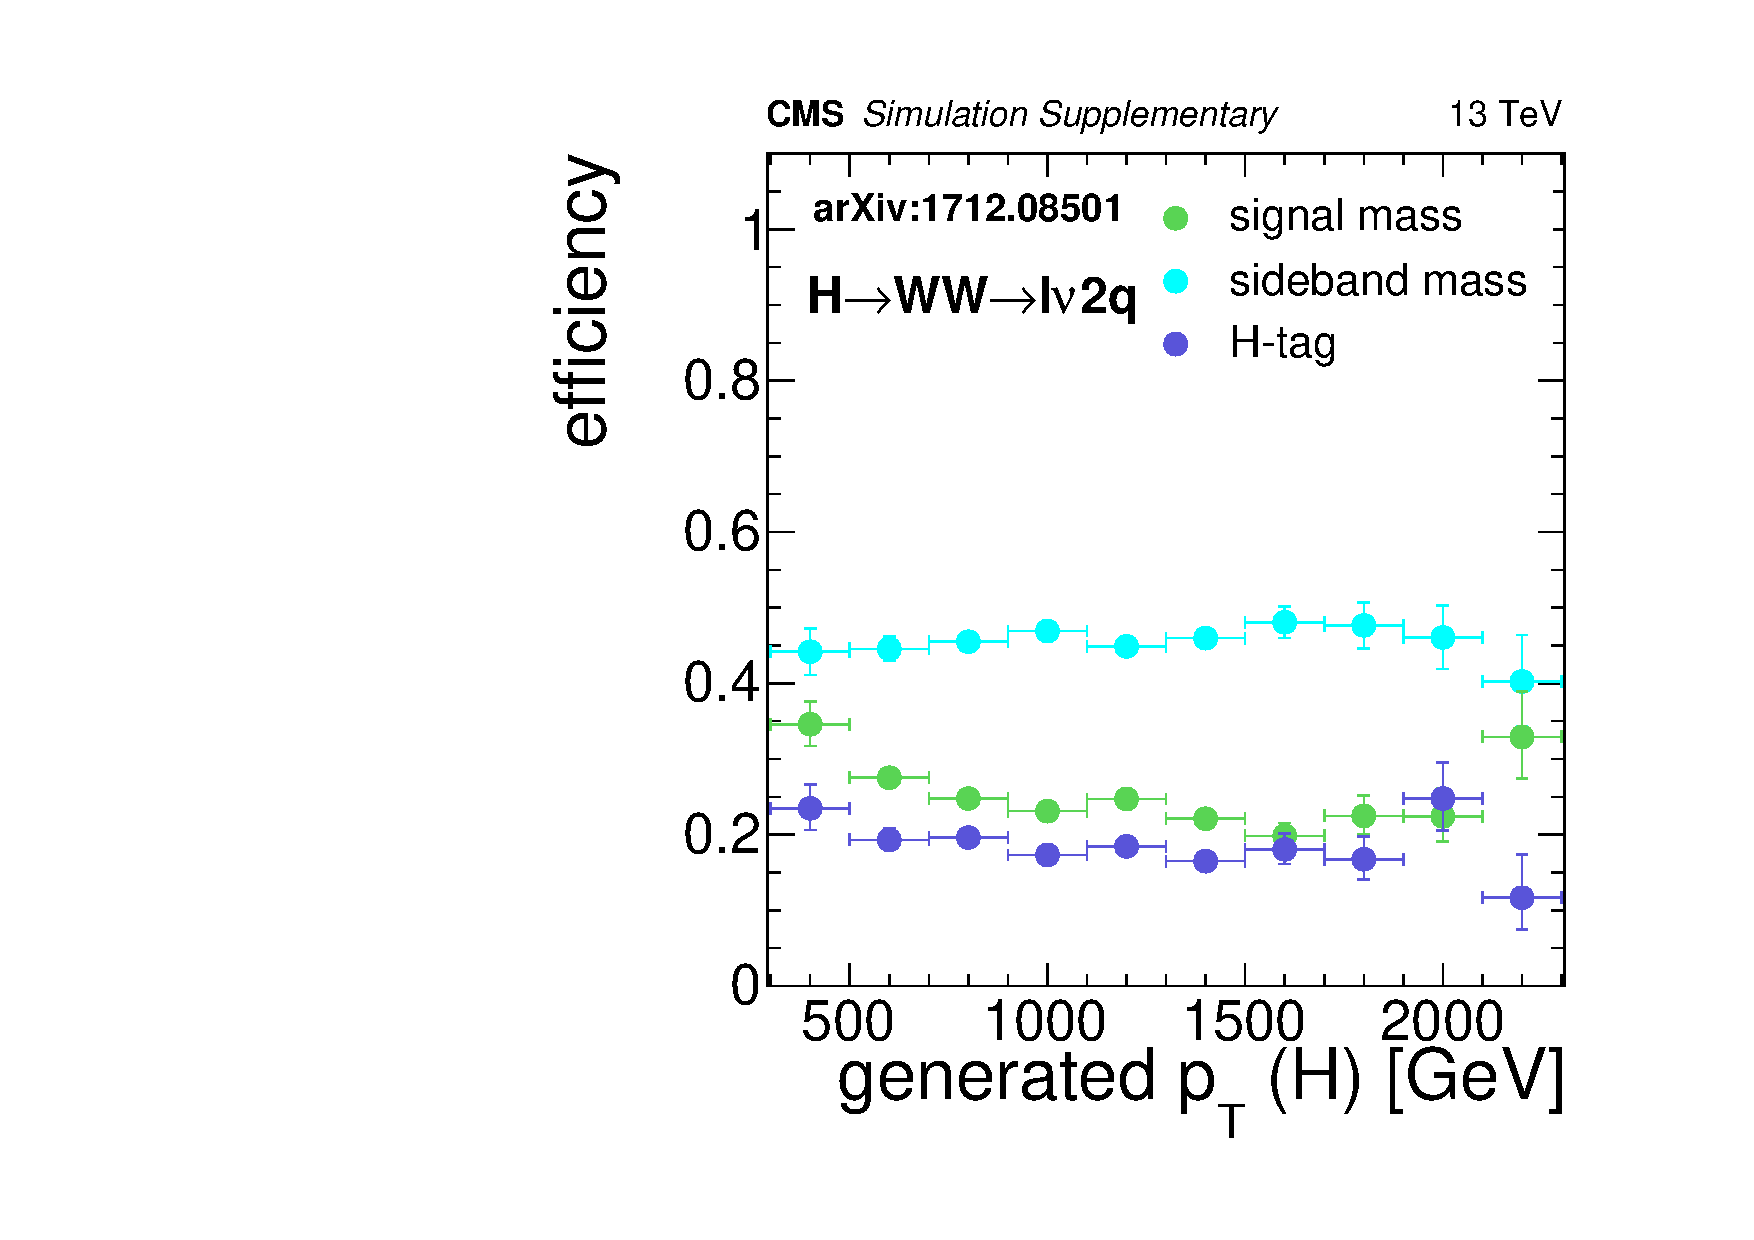
\includegraphics[width=0.425\linewidth]{figs/CMS-SUS-17-006_Figure-aux_008.pdf}
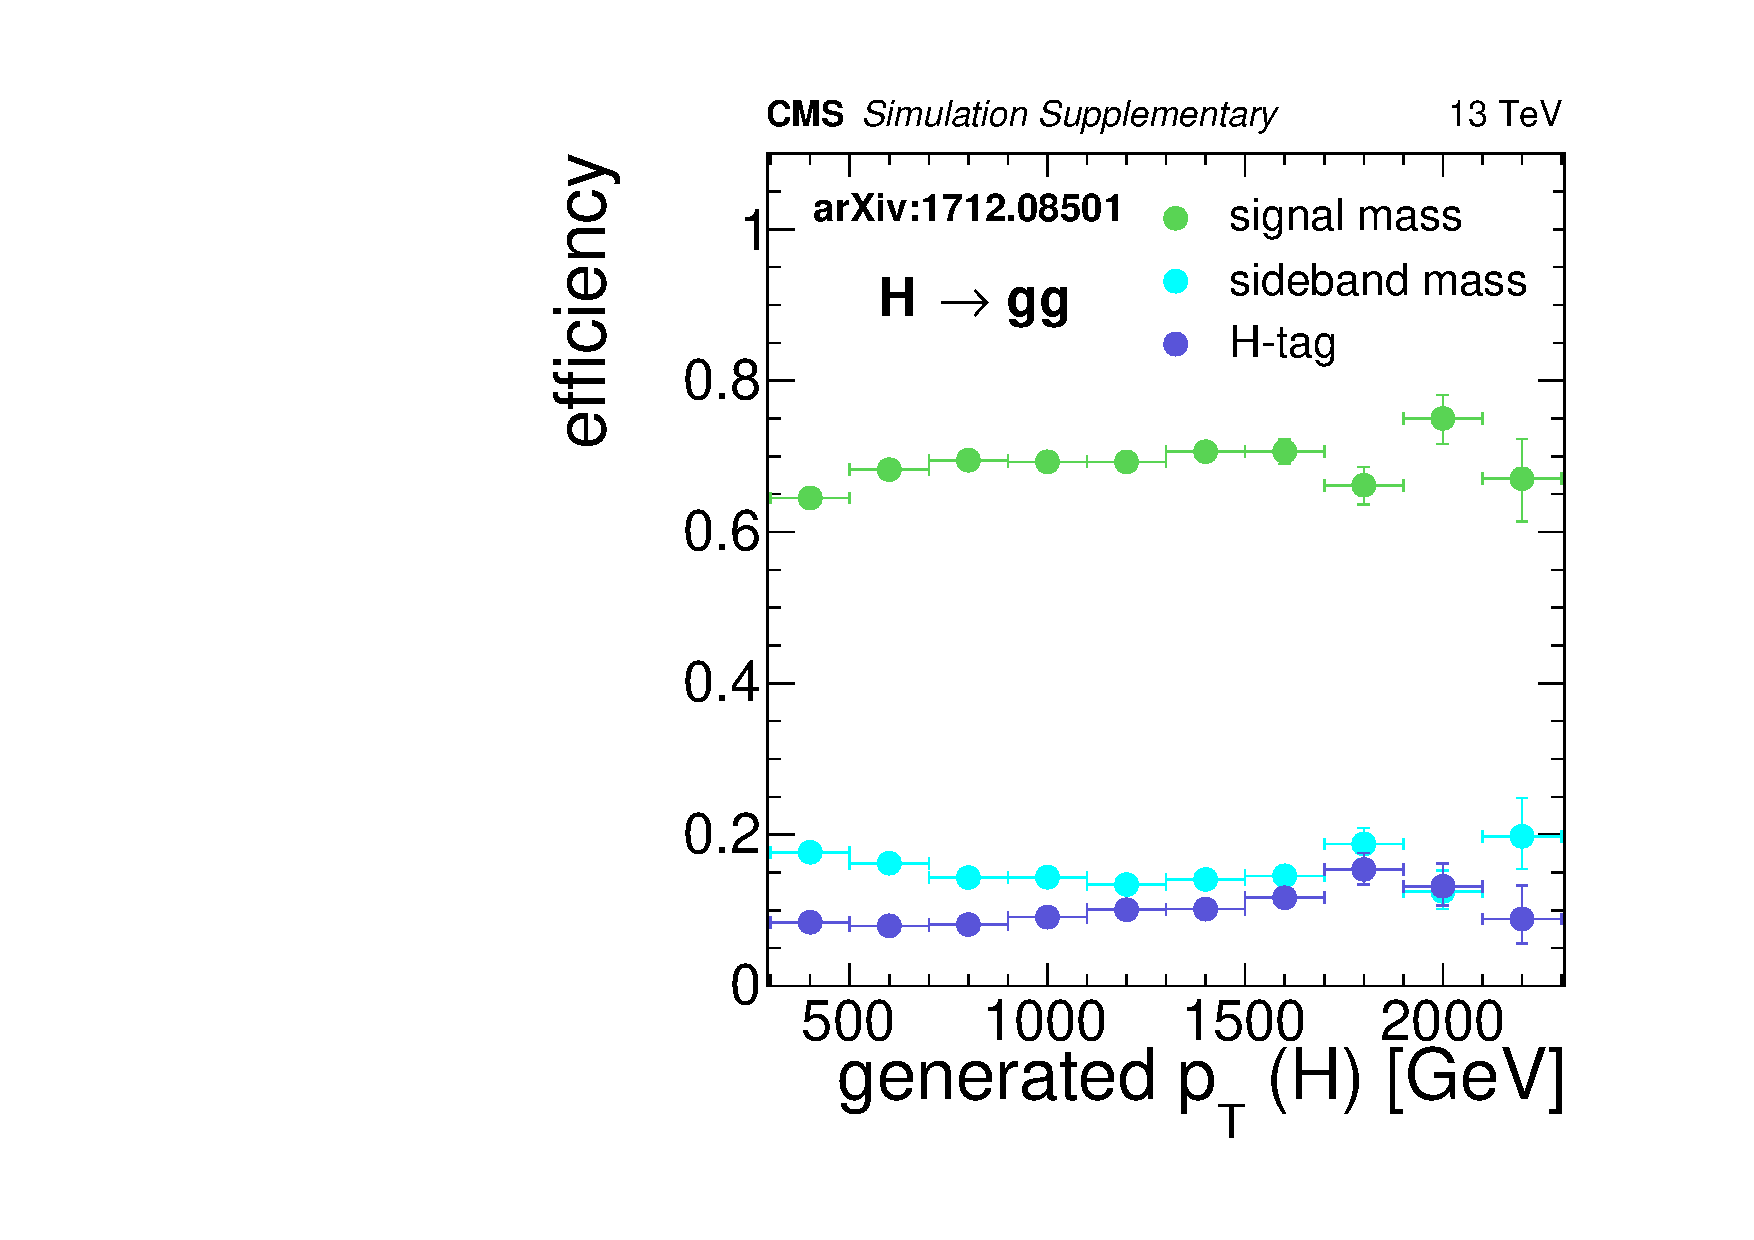
\includegraphics[width=0.425\linewidth]{figs/CMS-SUS-17-006_Figure-aux_009.pdf}
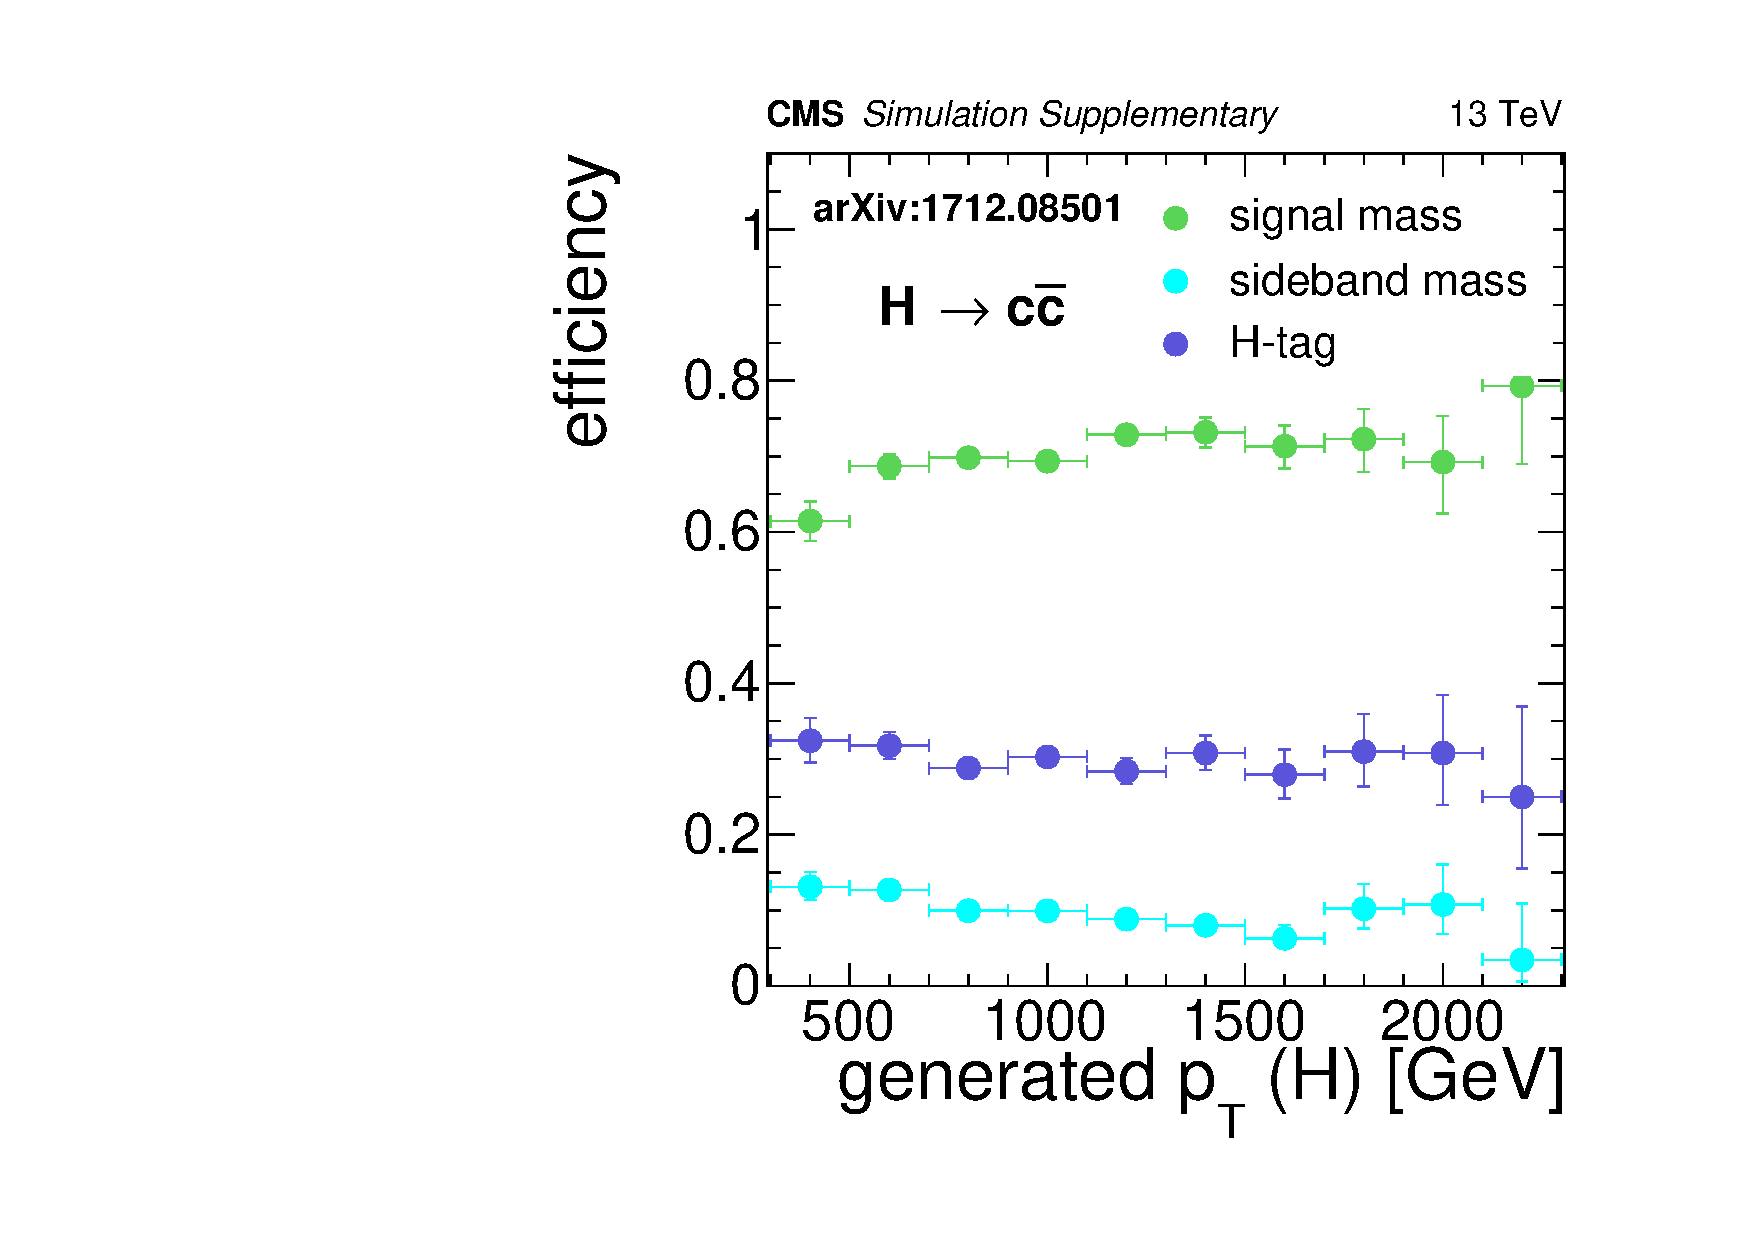
\includegraphics[width=0.425\linewidth]{figs/CMS-SUS-17-006_Figure-aux_010.pdf}

\includegraphics[width=0.425\linewidth]{figs/blankcanvas.pdf}
\caption
[Efficiencies for an AK8 jet originating from H boson decay, relative to baseline selection.]
{Efficiencies for an AK8 jet originating from H boson decay, relative to baseline selection. "signal mass" represents the probability the jet will have mass [85, 135 GeV]. "sideband mass" represents the probability the jet will have mass [50, 85 GeV] or [135, 250 GeV]. "H-tag" represents the probability the jet have a double-b discriminator value greater than 0.3, for jets with mass [50, 250 GeV]. Efficiencies were derived using the T5ZH  with a gluino mass of 2200 GeV. }
\label{fig:effH}
\end{figure}

\begin{figure}[hbp!]
\centering
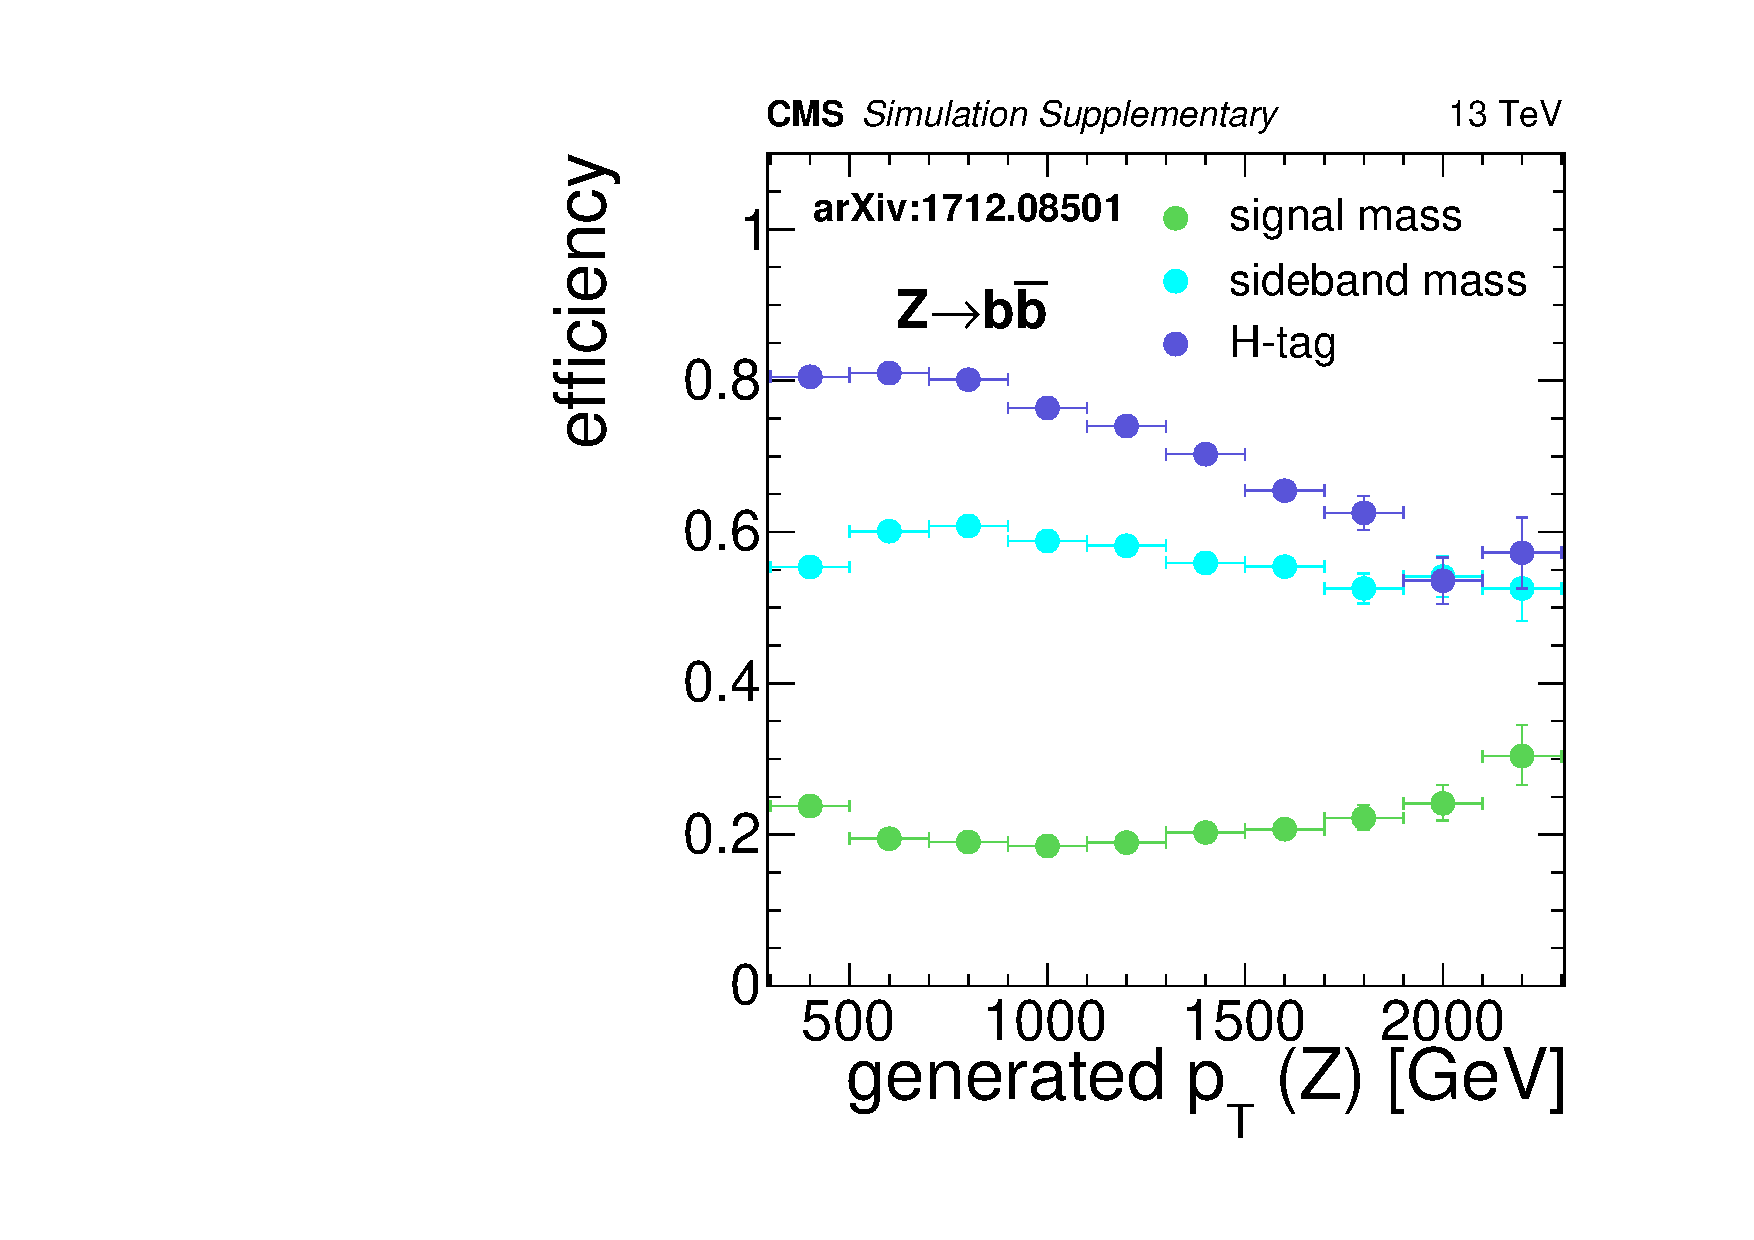
\includegraphics[width=0.425\linewidth]{figs/CMS-SUS-17-006_Figure-aux_011.pdf}
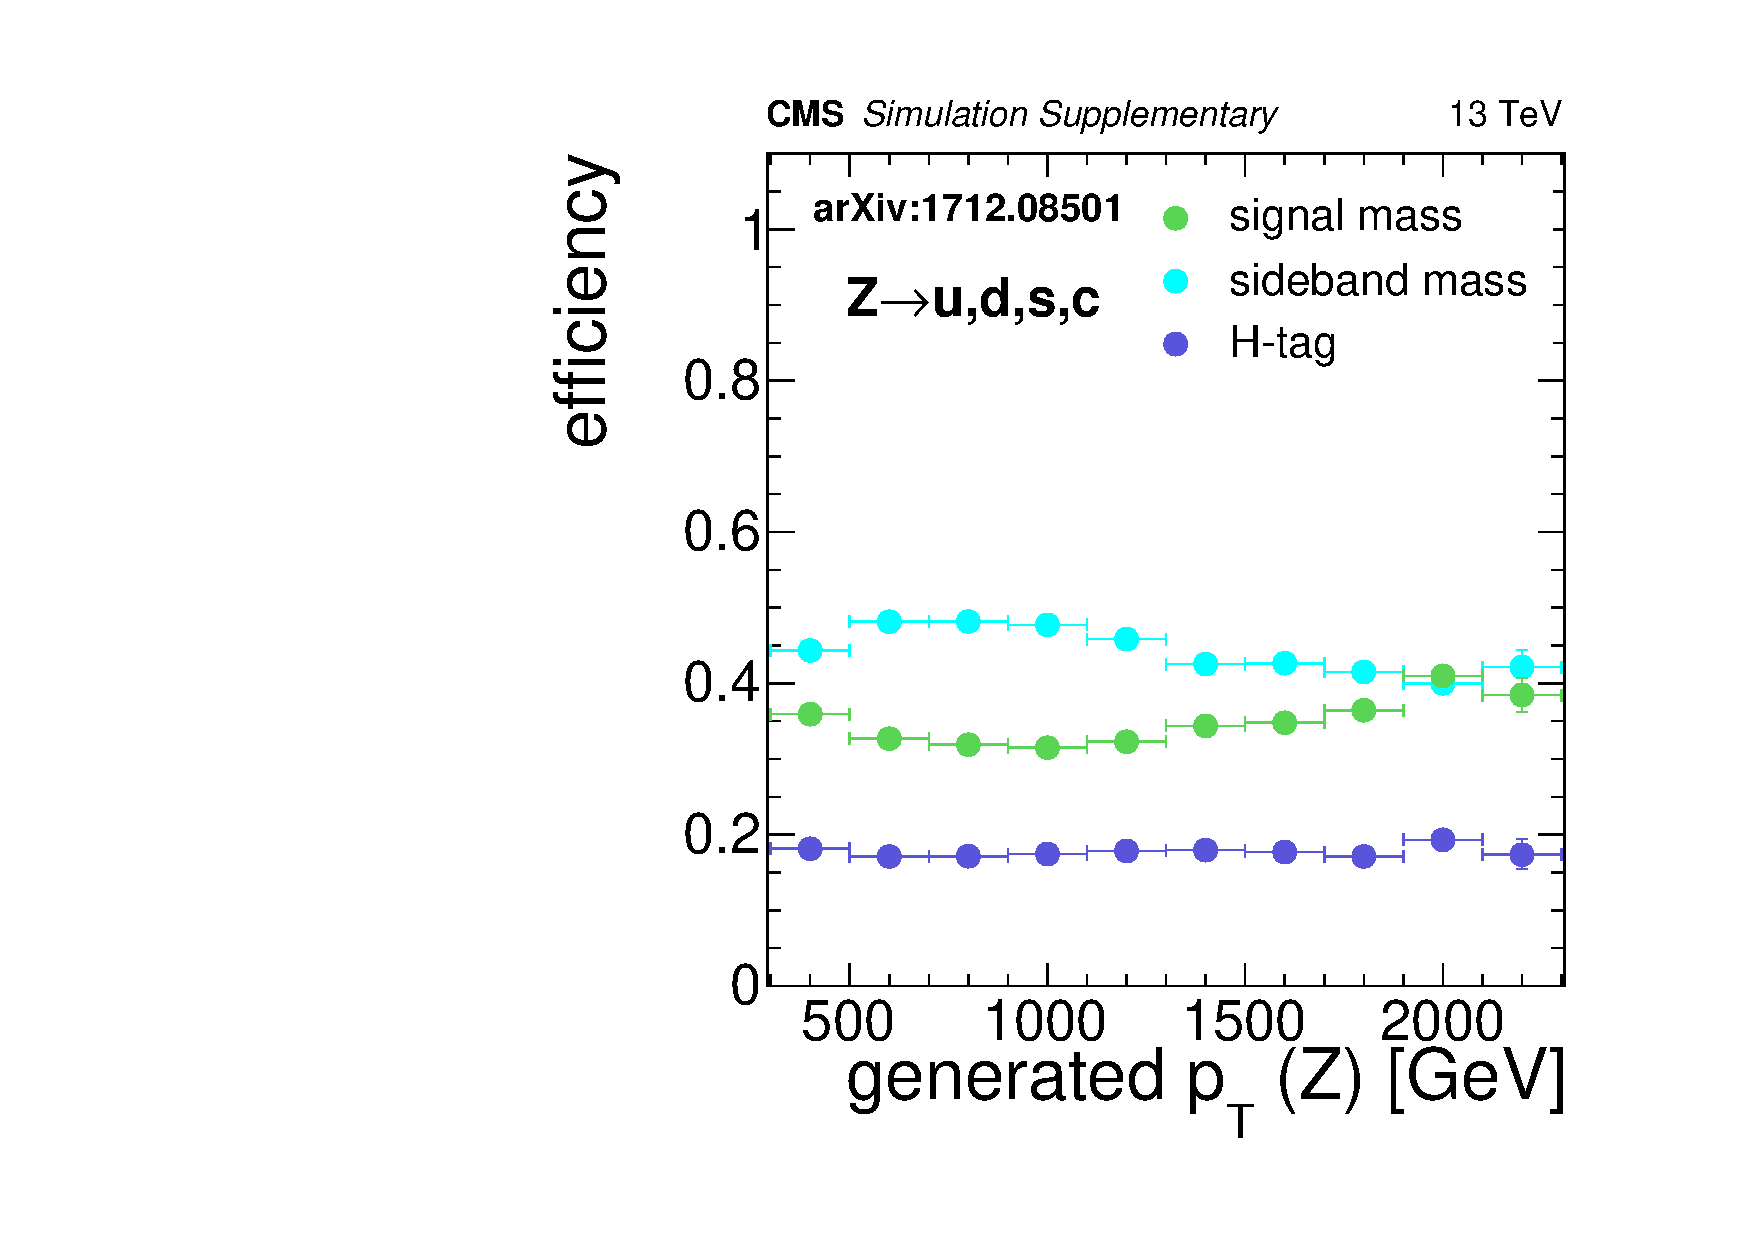
\includegraphics[width=0.425\linewidth]{figs/CMS-SUS-17-006_Figure-aux_012.pdf}
\caption[Efficiencies for an AK8 jet originating from Z boson decay, relative to baseline selection.]
{Efficiencies for an AK8 jet originating from Z boson decay, relative to baseline selection. "signal mass" represents the probability the jet will have mass  [85, 135 GeV]. "sideband mass" represents the probability the jet will have mass [50, 85 GeV] or [135, 250 GeV]. "H-tag" represents the probability the jet have a double-b discriminator value greater than 0.3, for jets with mass [50, 250 GeV]. Efficiencies were derived using the T5ZH  with a gluino mass of 2200 GeV.
}
\label{fig:effZ}
\end{figure}

As a test of closure, the prescription is tested using the T5HH model with a gluino mass of 2200 GeV. The yields in each of the 6 analysis bins for this model point (inclusive in \ptmiss) are listed in Table~\ref{tab:predclos} under the heading ``RECO truth''. As the efficiency maps are $p_{T}$ dependent, we have the choice of using the momentum of the reconstructed or the generated bosons. The ``RECO prediction'' column in the table uses the reconstructed momentum as input, ``GEN prediction'' uses the generated momentum. The largest deficit is in the D region, with a difference of -36\% difference from nominal. The greatest over-prediction is found in the B2 region, with a surplus of +8.2\% events relative to nominal. The closure in the other bins fall somewhere in this range.

\begin{table}[hbp!]
\centering
\caption[Comparison of the event yields in the 6 analysis regions with those obtained via the prediction.]{
Comparison of the event yields in the 6 analysis regions with those obtained via the prediction. The prediction was made using the T5HH signal MC with a gluino mass of 2200 GeV.
}
\begin{tabular}{c | c c c}
\hline\hline
         & RECO & RECO           & GEN\\
         & ``truth''             & prediction     & prediction\\
\hline
Baseline & 4.08     & 3.46 (${-}15\%$)   & 3.53 (-16\%)\\
A1       & 1.21     & 1.18 (-2.3\%)  & 1.26 (+3.6\%)\\
A2       & 0.777    & 0.748 (-3.7\%) & 0.815 (+4.7\%)\\
B1       & 0.802    & 0.703 (-12\%)  & 0.664 (-21\%)\\
B2       & 0.322    & 0.338 (+5.0\%) & 0.350 (+8.2\%)\\
C        & 0.498    & 0.473 (-4.9\%) & 0.487 (-2.1\%)\\
D        & 0.478    & 0.353 (25\%)   & 0.308 (-36\%)\\
\hline\hline
\end{tabular}
\label{tab:predclos}
\end{table}

%\begin{table}[hbp!]
%\centering
%\caption
%[T5HH/ZH signal event cutflow.]
%{T5HH and T5ZH signal efficiencies cutflow for two different gluino masses. The first row represents no selection, the final row represents the selection for the ``A$_{2}$'' signal event bin of the main analysis (inclusive in $p_{T}$).
%}
%\label{tab:}
%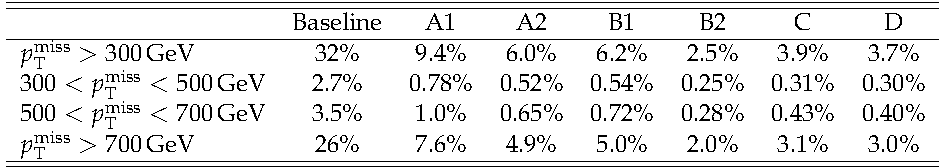
\includegraphics[width=0.9\linewidth]{figs/CMS-SUS-17-006_Table-aux_003.pdf}
%\end{table}
%
%\begin{table}[hbp!]
%\centering
%\caption[T5HH signal event efficiencies.]{
%Signal efficiencies for an event to land in a given analysis bin.
%The efficiencies were derived using the T5HH with a gluino mass of 2200 GeV.
%Choosing a gluino mass of 1800 GeV decreases the efficiencies by a relative 5\%.
%}
%\label{tab:sigeff}
%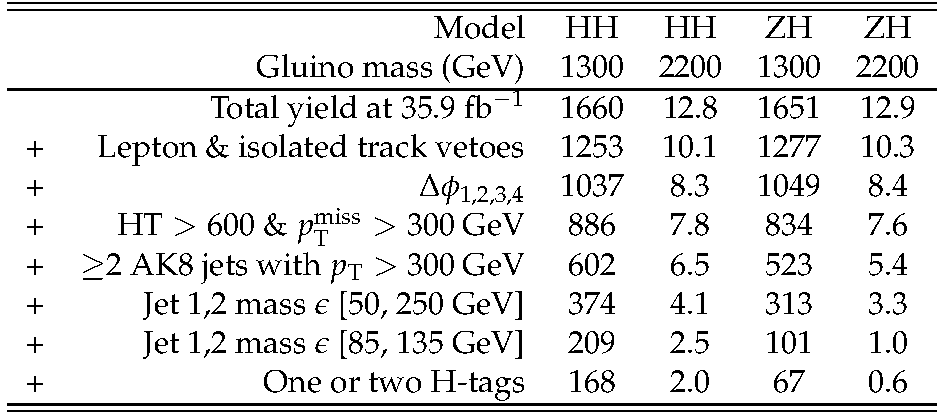
\includegraphics[width=0.9\linewidth]{figs/CMS-SUS-17-006_Table-aux_002.pdf}
%\end{table}
